\usepackage{extarticle}
\documentclass[14pt]{extarticle}
\usepackage[paperheight=8.7in, paperwidth=11in, total={10.5in, 8.2in}]{geometry}
\usepackage{tikz}

\usetikzlibrary{automata, positioning, shapes.geometric, arrows.meta}

\tikzset{
    state/.style={
        ellipse, draw, fill={rgb:black,1;white,5},
        minimum size=10pt
    },
    mm/.style={
        -{Stealth[length=3mm]}
    },
    oo/.style={
        {Stealth[length=3mm]}-{Stealth[length=3mm]}
    },
    tikkup/.style={
        anchor=south west, rotate=27, align=left
    },
    tikkdown/.style={
        anchor=north east, rotate=27, align=right
    }
}

\begin{document}

\begin{center}
    {\Huge \bf Flowchart for Project Completion} \\[15pt]
    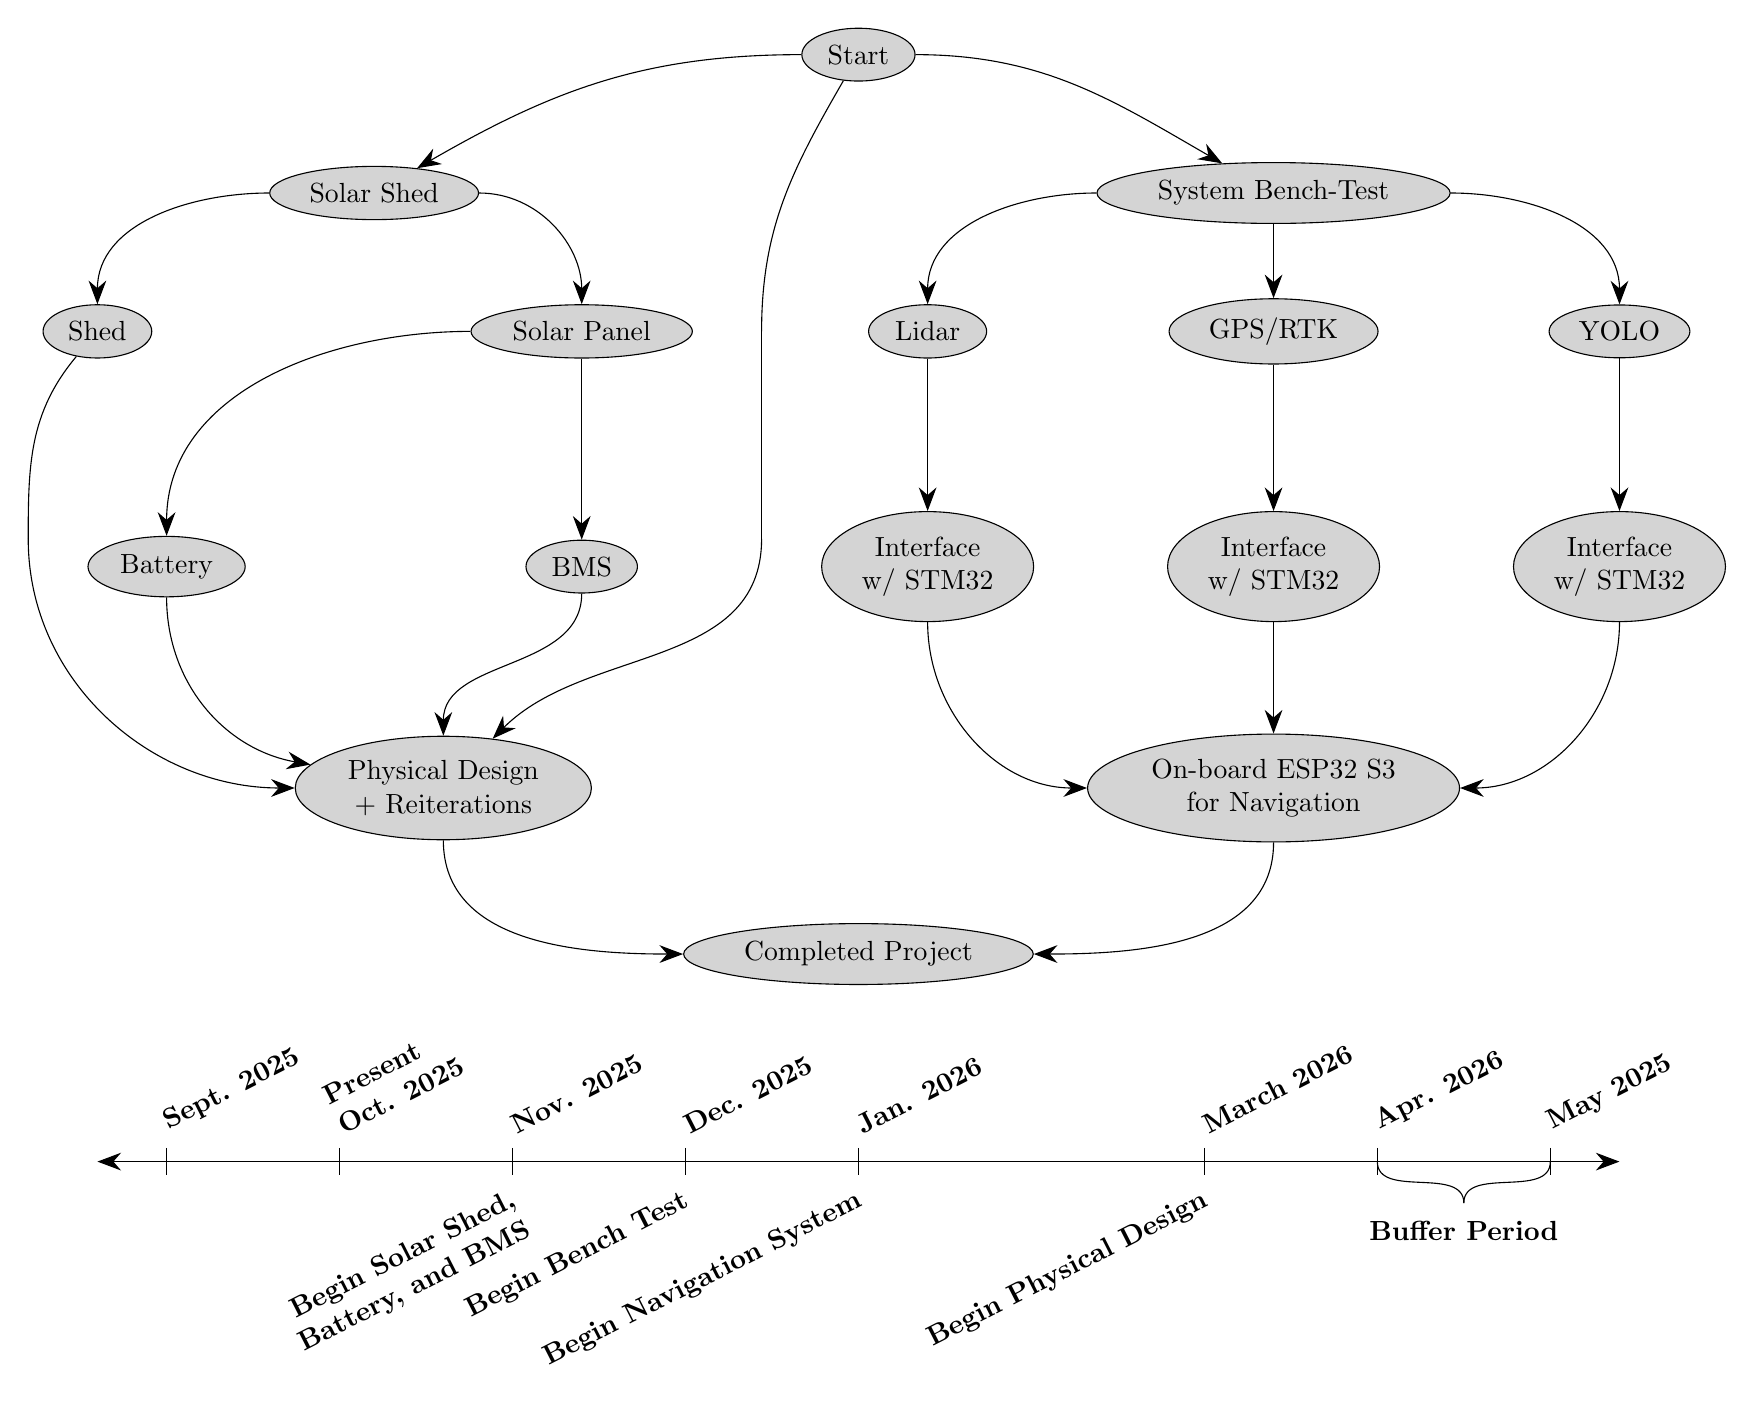
\begin{tikzpicture}[x=5pt, y=5pt]
        %\draw[help lines, step=5] (0,-30) grid (130,65);
        
        \node[state] (start)        at (65,60) {Start};
        
        \node[state] (SolarShed)    at (30,50) {Solar Shed};
        \node[state] (Shed)         at (10,40) {Shed};
        \node[state] (SolarPanel)   at (45,40) {Solar Panel};
        \node[state] (Battery)      at (15,23) {Battery};
        \node[state] (BMS)          at (45,23) {BMS};
        
        \node[state] (SystemBench) at (95,50) {System Bench-Test};

        \node[state] (Lidar)        at (70,40) {Lidar};
        \node[state] (GPS)          at (95,40) {GPS/RTK};
        \node[state] (YOLO)         at (120,40) {YOLO};
        % \node[state] (Triangle)     at (120,40) {Triangulation};

        \node[state, align=center] (Interface1)     at (70,23) {Interface\\w/ STM32};
        \node[state, align=center] (Interface2)     at (95,23) {Interface\\w/ STM32};
        \node[state, align=center] (Interface3)     at (120,23) {Interface\\w/ STM32};

        \node[state, align=center] (Navigation) at (95,7) {On-board ESP32 S3\\for Navigation};

        \node[state, align=center] (physical) at (35,7) {Physical Design\\+ Reiterations};

        \node[state] (complete) at (65,-5) {Completed Project};

        \path (start) edge[mm, out=180, in=30] (SolarShed)
                (SolarShed) edge[mm, out=180, in=90] (Shed)
                (SolarShed) edge[mm, out=0, in=90] (SolarPanel)
                (SolarPanel) edge[mm, out=180, in=90] (Battery)
                (SolarPanel) edge[mm] (BMS)
                (start) edge[mm, out=0, in=150] (SystemBench)
                (SystemBench) edge[mm, out=-180, in=90] (Lidar)
                (SystemBench) edge[mm] (GPS)
                (SystemBench) edge[mm, out=0, in=90] (YOLO)
                %(SystemBench) edge[mm, out=0, in=90] (Triangle)
                (Lidar) edge[mm] (Interface1)
                (GPS) edge[mm] (Interface2)
                %(Triangle) edge[mm] (Feasible)
                %(Feasible) edge[mm, line width=2pt, dash pattern={on 6pt off 4pt}, out=-90, in=20] (Navigation)
                (YOLO) edge[mm, out=-90, in=90] (Interface3)
                (Interface3) edge[mm, out=-90, in=0] (Navigation)
                (start) edge[-, out=-120, in=90] (58,40)
                (58,40) edge[-, out=-90, in=90] (58,25)
                (58,25) edge[mm, out=-90, in=45] (physical)
                (physical) edge[mm, out=-90, in=180] (complete)
                (Navigation) edge[mm, out=-90, in=0] (complete)
                (Interface1) edge[mm, out=-90, in=180] (Navigation)
                (Interface2) edge[mm] (Navigation)
                (BMS) edge[mm, out=-90, in=90] (physical)
                (Battery) edge[mm, out=-90, in=170] (physical)
                (Shed) edge[-, out=-130, in=90] (5,25)
                (5,25) edge[mm, out=-90, in=180] (physical); 

        \draw[oo] (10,-20) -- (120,-20);

        % \node at (0,0) {O};
        
        \draw[-] (15,-19) -- (15,-21);
        \draw[-] (115,-19) -- (115,-21);
        \draw[-] (27.5,-19) -- (27.5,-21);
        \draw[-] (65,-19) -- (65,-21);
        \draw[-] (40,-19) -- (40,-21);
        \draw[-] (52.5,-19) -- (52.5,-21);
        \draw[-] (90,-19) -- (90,-21);
        \draw[-] (102.5,-19) -- (102.5,-21);

        \node[tikkup] at (15,-19) {\bf Sept. 2025};
        \node[tikkup] at (115,-19) {\bf May 2025};
        \node[tikkup] at (27.5,-19) {\bf Present\\\bf Oct. 2025};
        \node[tikkup] at (65,-19) {\bf Jan. 2026};
        \node[tikkup] at (40,-19) {\bf Nov. 2025};
        \node[tikkup] at (52.5,-19) {\bf Dec. 2025};
        \node[tikkup] at (90,-19) {\bf March 2026};
        \node[tikkup] at (102.5,-19) {\bf Apr. 2026};

        \node[tikkdown] at (40,-21) {\bf Begin Solar Shed,\\\bf Battery, and BMS};
        \node[tikkdown] at (52.5,-21) {\bf Begin Bench Test};
        \node[tikkdown] at (65,-21) {\bf Begin Navigation System};
        \node[tikkdown] at (90,-21) {\bf Begin Physical Design};

        \path (102.5,-20) edge[out=-90, in=90] (108.75,-23)
                (108.75,-23) edge[out=90, in=-90] (115,-20);

        \node at (108.75,-25) {\bf Buffer Period};
    \end{tikzpicture}
\end{center}
    
\end{document}